\documentclass[]{beamer}
\usepackage[utf8]{inputenc}
\usepackage[T1]{fontenc}
\usepackage{carlito}
\usetheme[horizontal=true, hr=false, pagenumbers=true]{NewPwr}
\usepackage{bibentry}
\usepackage{minted}
\setminted{fontsize=\small,baselinestretch=1}
\usepackage{multicol}
\usepackage{polski}

% Build-specific command
\nonstopmode

%Information to be included in the title page:
\title{Przewidywanie zapotrzebowania na energię na podstawie danych \textit{PJM Interconnection LLC}}
\subtitle{Przedmiot Monograficzny -- projekt}
\author{Mateusz Bączek, Michał Rajkowski, Konrad Bratek}
\institute{Politechnika Wrocławska}
\date{2023}

\begin{document}

\frame{\titlepage}

\section{Wstęp teoretyczny}

\begin{frame}
\frametitle{Zbiór danych -- PJM Interconnection LLC}
  \begin{figure}
    \centering
    
\includegraphics[width=0.3\linewidth]{pjm-logo.png}
    \caption{Logo \textit{PJM interconnection}}
  \end{figure}
  \vspace{-0.5cm}
  \begin{figure}
    \centering
    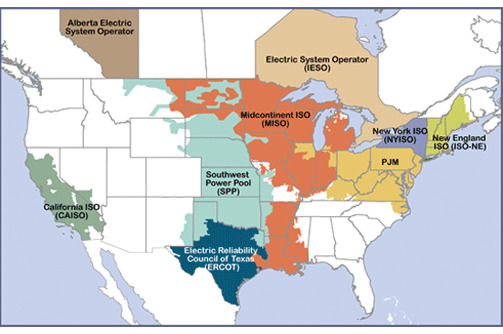
\includegraphics[width=0.6\linewidth]{rto_map.jpg}
    \caption{Operatorzy sieci elektrycznej na terenie Stanów Zjednoczonych.}
  \end{figure}

\end{frame}

\begin{frame}
\frametitle{PJM Interconnection LLC}
% \vspace{-1cm}
  \textbf{Z informacji o zbiorze danych, który znaleźliśmy:} \\
  \begin{quote}
Interconnection grid operating an electric transmission system serving all or parts of Delaware, Illinois, Indiana, Kentucky, Maryland, Michigan, New Jersey, North Carolina, Ohio, Pennsylvania, Tennessee, Virginia, West Virginia, and the District of Columbia.
  \end{quote}

  \begin{figure}
    \centering
    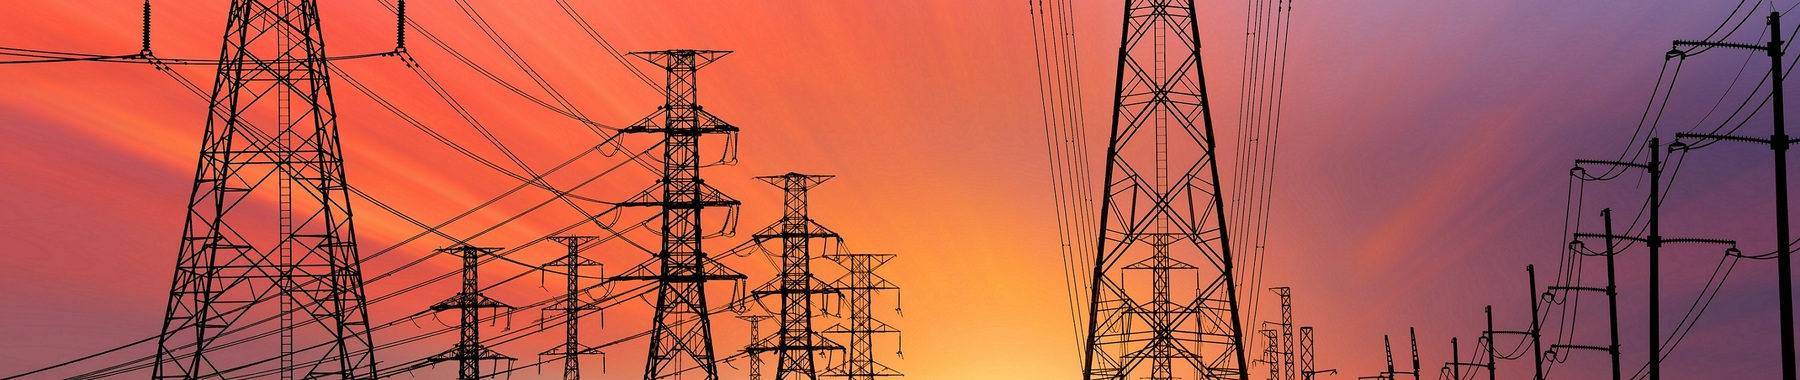
\includegraphics[width=0.8\linewidth]{dataset-cover.jpg}
    % \caption{Grafika reklamowa firmy \textit{Elastic}, tworzącej rozwiązania monitorujące.}
  \end{figure}

\end{frame}

\begin{frame}
\frametitle{Cele projektu}
\vspace{-1cm}


\begin{enumerate}
  \item Przewidywanie zużycia energii na dzień do przodu,
  \item testy przewidywania w dłuższej perspektywie czasowej (kilka dni/tydzień),
  \item sprawdzenie trendów zużycia energii podczas świąt, wakacji, itd.
  \item przetestowanie skuteczności różnych modeli predykcyjnych,
  \item przetestowanie sprawności modelu na danych od innego dostawcy energetycznego (jeśli uda się znaleźć).
\end{enumerate}
\end{frame}

\section{Bibliografia}

\begin{frame}
  \centering
  \huge{
    Dziękujemy za uwagę!}
\end{frame}

% \begin{frame}
%   \begin{thebibliography}{99} % Beamer does not support BibTeX so references must be nserted manually as below
%   \bibitem[Pourmajidi, 2023]{ibm} Pourmajidi, William and Zhang, Lei and Steinbacher, John and Erwin, Tony and Miranskyy, Andriy (2023)
%   \newblock A Reference Architecture for Observability and Compliance of Cloud Native Applications
%   \newblock \emph{Toronto Metropolitan University, University of Maryland, Baltimore County, USA, IBM Canada Lab, Toronto, Canada, IBM Cloud Platform, Austin, USA}
%   \newblock \url{https://www.gartner.com/smarterwithgartner/how-to-start-an-it-monitoring-initiative}

%   \bibitem[Perri, 2022]{gartner} Lori perri (2022)
%   \newblock Monetizing Observable Data Will Separate the Winners and Losers
%   \newblock \emph{Gartner Insights}
%   \newblock \url{https://gartner.com/en/articles/monetizing-observable-data-will-separate-the-winners-and-losers}

%   \end{thebibliography}
% \end{frame}

% \begin{frame}
%   \begin{thebibliography}{99} % Beamer does not support BibTeX so references must be nserted manually as below
%   \bibitem[Shetty, 2017]{gartner2} Sony Shetty (2017)
%   \newblock How to Start an IT Monitoring Initiative
%   \newblock \emph{Gartner Insights}
%   \newblock \url{https://www.gartner.com/smarterwithgartner/how-to-start-an-it-monitoring-initiative}

%   \end{thebibliography}
% \end{frame}

\end{document}

